\documentclass{article}
\usepackage[hmargin=1.5cm,vmargin=1.5cm]{geometry}

\usepackage{listings}
\usepackage{color}
\usepackage{graphicx}
\usepackage{float}
\usepackage{amsmath}
\usepackage{subfig}
\usepackage{cite}
\usepackage{url}
\usepackage{amsmath}

\newcounter{qcounter}

\begin{document}

\title{Image Analysis - TP6 - Background Subtraction}

\author{Jander Nascimento, 
\and Raquel Oliveira}

\maketitle

\section{Introduction}

The goal of segmentation is to simplify and/or change the representation of an image into something that is more meaningful and easier to analyze. Image segmentation is the process of assigning a label to every pixel in an image such that pixels with the same label share certain visual characteristics.\cite{introduction}

Segmentation is mostly used for object recognition, differentiate those objects from the background, image compression or image editing.

In this practical work, we implemented an approach for image segmentation for background subtraction, with which is possible to identify the foreground region in an image given a set of images of the background.


\section{The method}

In this exercise we use a Gaussian model to build a statistical model of the background for each pixel in the image. For each colored pixel \textit{i}, i.e., \textit{i=($i_r, i_g, i_b$)}, the probability density applied is described in equation \ref{equa:themethod}:

\begin{equation}
	p_b(i)=\frac{1}{(2\pi)^{\frac{3}{2}}|\Sigma|^{\frac{1}{2}}}exp(\frac{-1}{2}(i-i_m)^T\Sigma^{-1}(i-i_m))
\label{equa:themethod}
\end{equation}

where {$i_m$} is the mean value with respect to the given set of \textit{N} values {$i_n$}:

\begin{equation}
	i_m = \frac{1}{N}\sum_{n=1}^{N}{i_n}
\end{equation}

and {$\Sigma$} is the covariance matrix:

\begin{equation}
	\Sigma = \frac{1}{N}\sum_{n=1}^{N}({i_n}-{i_m})({i_n}-{i_m})^T
\end{equation}


\section{Results}
We implemented the equation \ref{equa:themethod} step by step. First creating all the methods that would be useful to generate the model, as subtraction and multiplication between matrices; transpose, inverse and determinant of a matrix and the covariance matrix.

We calculate the mean matrix once, in the beginning of the method. Over there we stored the mean value for each pixel (\textit{$i_m$} in the formula above) with respect to their colors in all the background images considered.

With the previous methods was possible to build the Gaussian model for all pixels in the images in the background. We were given 115 images of the static background, to build the model (Figure \ref{background}).

	\begin{figure} [H]
		\centering
		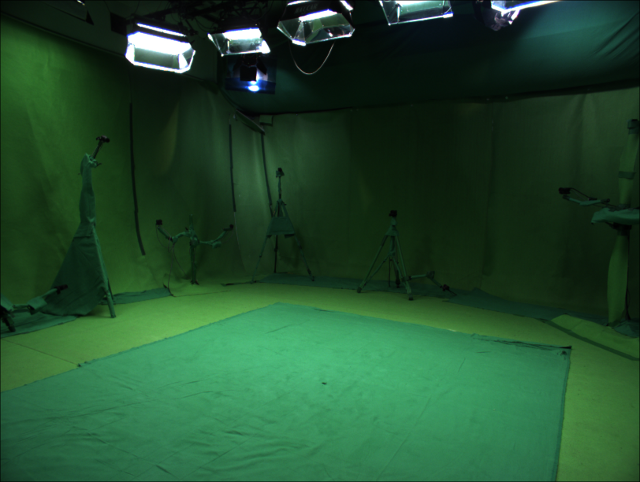
\includegraphics[scale=0.3]{img/img_000000}
		\caption{Example of background\label{background}}
	\end{figure}

	We tested the statistical model with the 5 given foreground images. For each pixel, based on the model, we can determine if the pixel belongs either to a foreground or to a background of the image.

	Given an input image with a foreground, we create a binary image with two regions: foreground and background. What determines which region the pixel belongs to is the probability given by the Gaussian model. To do so, it is needed to threshold the probability for each pixel.

	The probability that a pixel belongs to a background is given by the formula described in equation \ref{equa:themethod}. And the probability that a pixel belongs to a foreground is:

	\begin{equation}
	 p_f(i)=1-p_b(i)  
	\end{equation}

	We tested some thresholds to determine which one would be more suitable to properly distribute the pixels in the 2 regions, and the value that gave better results was 0.01. So, if {$p_b(i)>0,01$}, means that the pixel belongs to the background (which we painted in black). Otherwise, it belongs to the foreground (which we painted in white). 

	We can see in Figure \ref{fig:img_000053} the results of the algorithm for a image with a foreground. To obtain this result, all the 115 background images were used to built the statistical model.

	\begin{figure}[H]
		  \centering
		  \subfloat[Original Image]{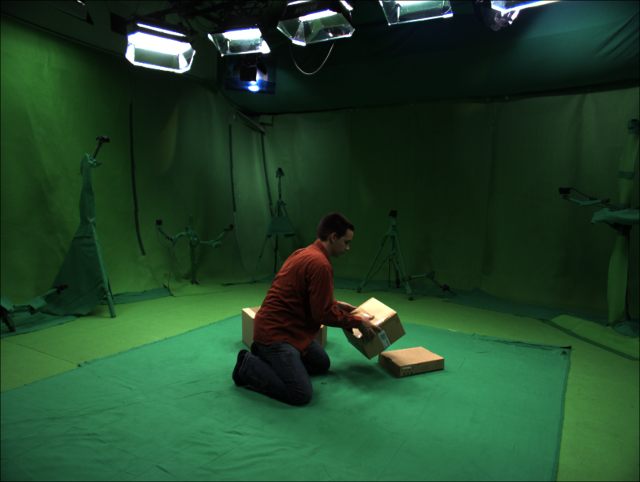
\includegraphics[width=0.3\textwidth]{img/img_000053}}                
		  \subfloat[Binary Image]{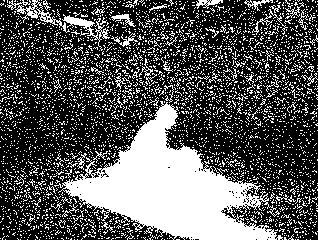
\includegraphics[width=0.3\textwidth]{img/result_53_115}}
		  \caption{Background Subtraction}
		  \label{fig:img_000053}
	\end{figure}

\subsection{Effect of the threshold}

	We observed that the lower the threshold is, the better is the result achieved. In the Figure \ref{fig:threshold} we can see the effect of different thresholds (denoted by T) with the same number of background images (115).

	We used the threshold in the following way:

	\begin{lstlisting}[frame=single]
		T:=0.01
		IF p(i)>T
			pixel belongs to background
		ELSE
			pixel belongs to foreground
		
	\end{lstlisting}

	\begin{figure}[H]
		  \centering
		  \subfloat[Original Image]{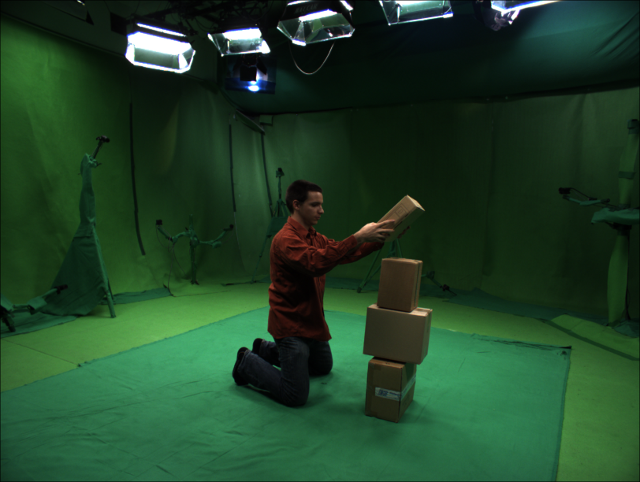
\includegraphics[width=0.2\textwidth]{img/img_000348}}
		  \subfloat[T=0,5]{
\includegraphics[width=0.2\textwidth]{img/result_348_115-50}}
		  \subfloat[T=0,1]{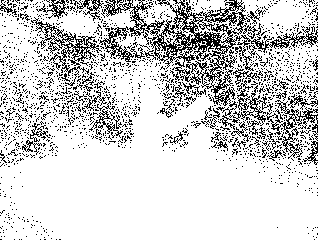
\includegraphics[width=0.2\textwidth]{img/result_348_115-10}}
		  \subfloat[T=0,01]{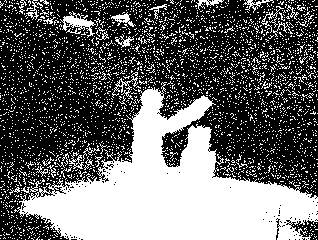
\includegraphics[width=0.2\textwidth]{img/result_348_115}}
		  \caption{Effect of the threshold (T)}
		  \label{fig:threshold}
	\end{figure}

\subsection{Effect of the number of background images}

	We observed that the more static background images you use to build the statistical model, better the result is. Which means that the pixels will be more correctly classified in their segments. We illustrate this in the Figure \ref{fig:nback}, with different number of background images being used (denoted by N). However, the computational cost increases proportionally with the number of background images used to build the statistic model.

	\begin{figure}[H]
		  \centering
		  \subfloat{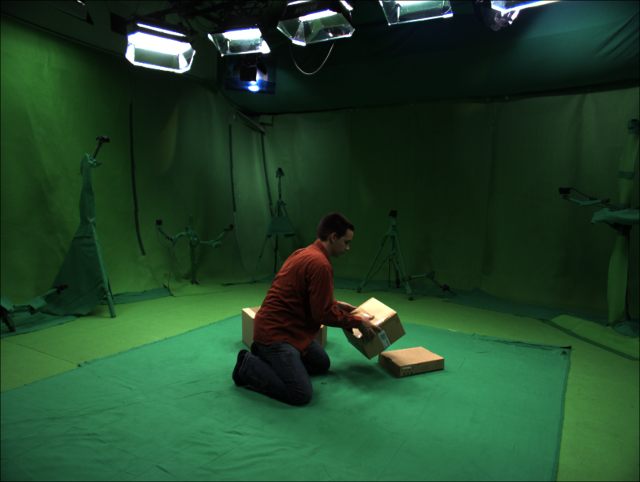
\includegraphics[width=0.2\textwidth]{img/img_000053}}
		  \subfloat{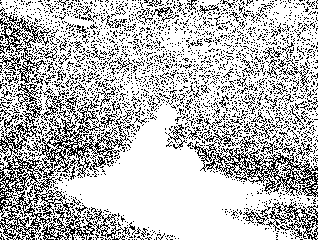
\includegraphics[width=0.2\textwidth]{img/result_53_5}}
		  \subfloat{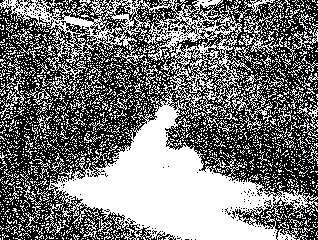
\includegraphics[width=0.2\textwidth]{img/result_53_15}}
		  \subfloat{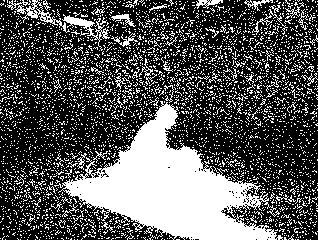
\includegraphics[width=0.2\textwidth]{img/result_53_115}}
		  \hspace{0.1cm}
		  \subfloat{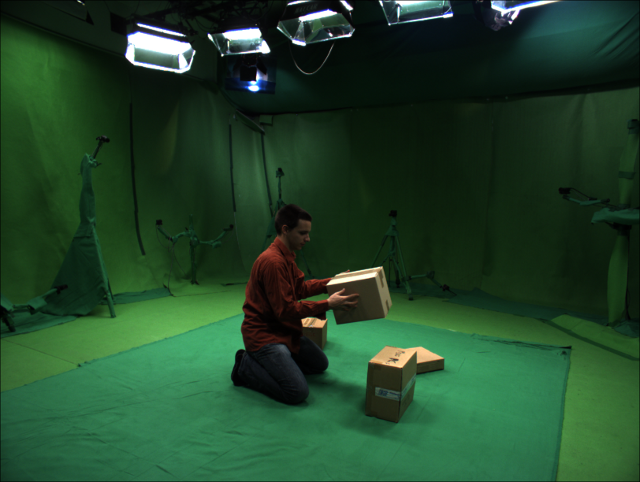
\includegraphics[width=0.2\textwidth]{img/img_000147}}                
		  \subfloat{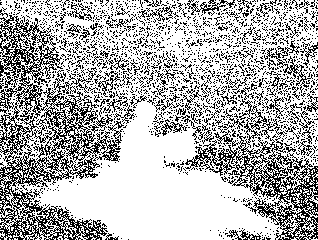
\includegraphics[width=0.2\textwidth]{img/result_147_5}}
		  \subfloat{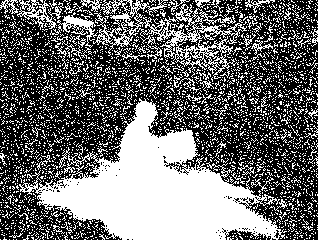
\includegraphics[width=0.2\textwidth]{img/result_147_15}}
		  \subfloat{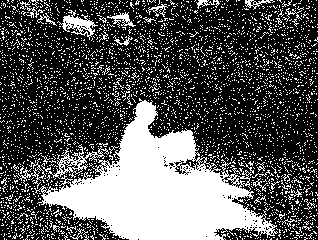
\includegraphics[width=0.2\textwidth]{img/result_147_115}}
		  \hspace{0.1cm}
		  \subfloat{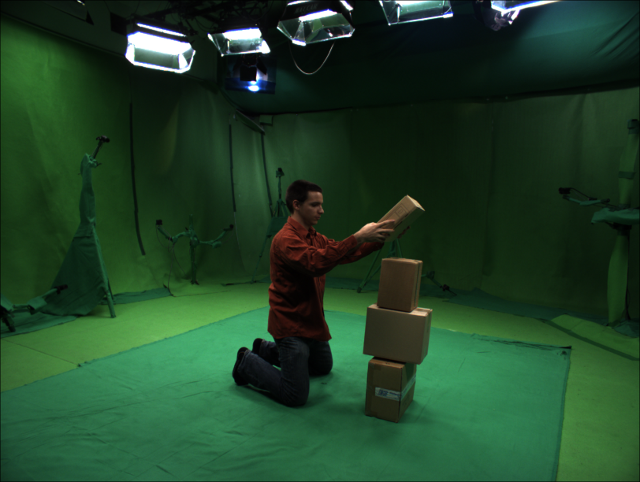
\includegraphics[width=0.2\textwidth]{img/img_000348}}
		  \subfloat{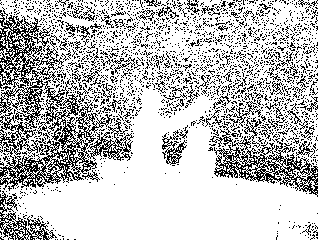
\includegraphics[width=0.2\textwidth]{img/result_348_5}}
		  \subfloat{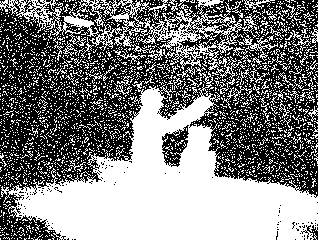
\includegraphics[width=0.2\textwidth]{img/result_348_15}}
		  \subfloat{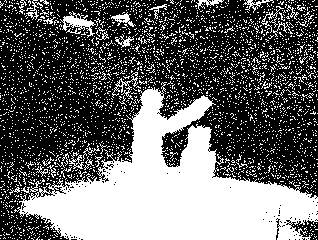
\includegraphics[width=0.2\textwidth]{img/result_348_115}}
		  \hspace{0.1cm}
		  \subfloat{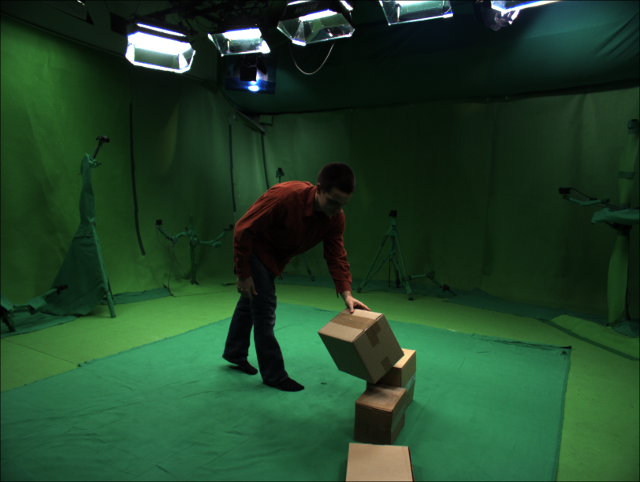
\includegraphics[width=0.2\textwidth]{img/img_000466}}
		  \subfloat{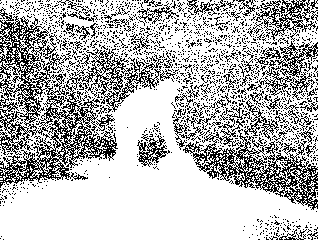
\includegraphics[width=0.2\textwidth]{img/result_466_5}}
		  \subfloat{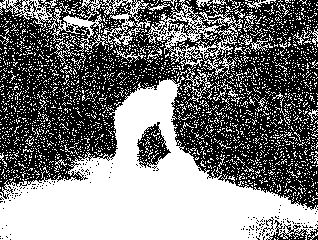
\includegraphics[width=0.2\textwidth]{img/result_466_15}}
		  \subfloat{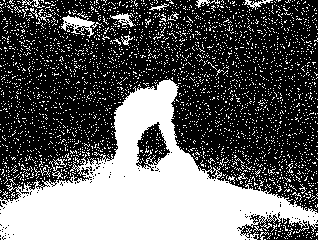
\includegraphics[width=0.2\textwidth]{img/result_466_115}}
		  \hspace{0.1cm}
		  \subfloat[Original Image]{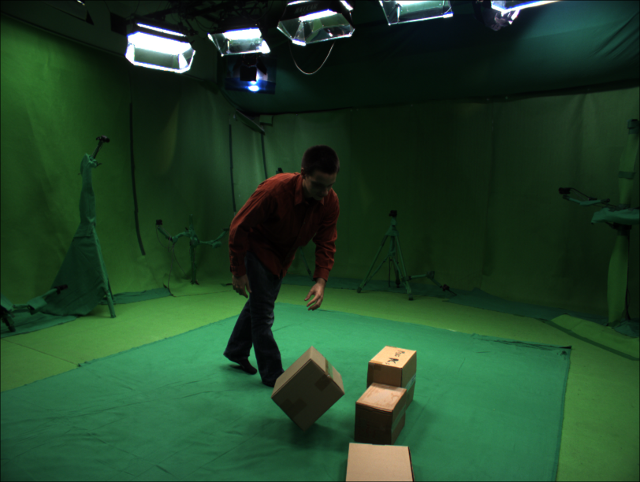
\includegraphics[width=0.2\textwidth]{img/img_000476}}
		  \subfloat[Binary Image N=5]{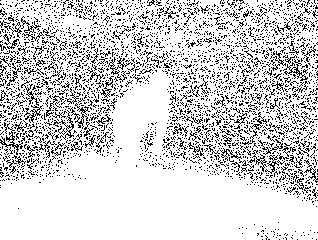
\includegraphics[width=0.2\textwidth]{img/result_476_5}}
		  \subfloat[N=15]{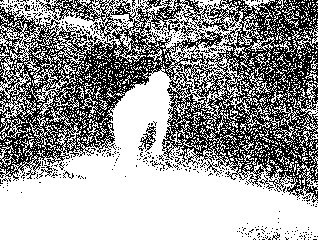
\includegraphics[width=0.2\textwidth]{img/result_476_15}}
		  \subfloat[N=115]{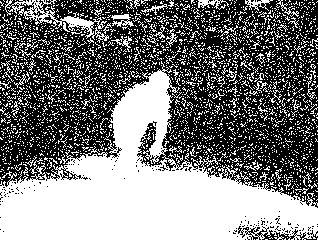
\includegraphics[width=0.2\textwidth]{img/result_476_115}}
		  \caption{Effect of the number of background images (N)}
		  \label{fig:nback}
	\end{figure}
	

\subsection{Comparison between the effects of the threshold and the number of background image}
	As said before, the computational cost of the algorithm increases proportionally with number of background images used to build the statistical model. To deal with this issue, it is possible to play with both parameters to improve the results. In the Figure \ref{thresxback} we show an example where both parameters are different. The image \ref{figure1} is the result of applying the algorithm with 115 background images, and a threshold equal to 0,06. To optimize the time, you could decrease the number of background images to 5 and also decrease the threshold to 0,01 (as in image \ref{figure2}), and the result will be equivalent.

	\begin{figure}[H]
		  \centering
		  \subfloat[Original Image]{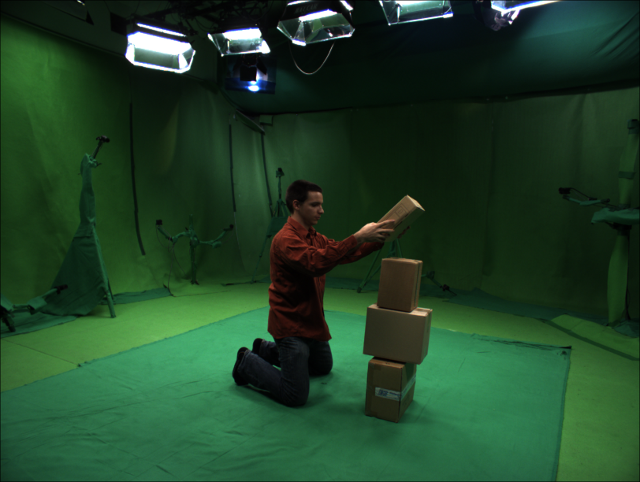
\includegraphics[width=0.3\textwidth]{img/img_000348}}
		  \subfloat[N=115 T=0,06]{\label{figure1}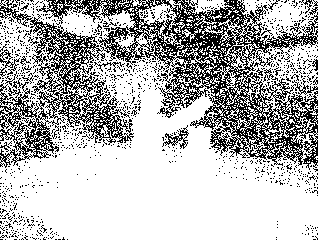
\includegraphics[width=0.3\textwidth]{img/result_348_115-6}}
		  \subfloat[N=5 T=0,01]{\label{figure2}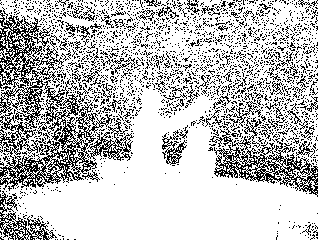
\includegraphics[width=0.3\textwidth]{img/result_348_5}}
		  \caption{Effect of both threshold (T) and number of backgrounds (N)}
		  \label{thresxback}
	\end{figure}
	
\section{Issues}
	This method consumes much memory. In order to build the Gaussian model, for each pixel of the foreground image all the background images are read, and each background is an image with dimensions 1224x1624, which leads to 1.987.776 pixels in memory for one single image. Since we are using all the 115 background images, in the end of the day it is necessary to keep in memory 228.594.240 pixels!

	As a consequence, the computation required to separate foreground and background is very high. The standard implementation we used so far to read ppm images was too slow to apply this method. Our read method by default reads the whole image and stores its pixels in a matrix(in memory), which we can use for any computation.

	To solve both problems of memory requirement and computation time, we changed our read image method to open a file and read the RGB values of only one pixel, instead of read and store all the pixels in a matrix, by calculating the position of the pixel inside a binary image file and positioning the file cursor in the exact pixel position. That change made possible to apply the method and achieve the results describe above.

	This was possible just because we converted the given images in a binary format of PPM, instead of the original PNG format.

\section{Equilikely foreground model}
	Without any particular knowledge of the foreground image colors, if we would like all colors to be equilikely in the foreground model, we could set:

	\begin{equation}
		p_f(i)=cst
	\end{equation}

	In order to achieve this, we should change the algorithm in the following way: instead of calculate the equation \ref{equa:themethod} to build the Gaussian model, we just threshold {$p_f$} with a constant value \textit{cst}, and set {$p_b$} to be:

	\begin{equation}
	 p_b(i)=1-p_f(i)  
	\end{equation}
	
\section{How to run?}

	Steps to compile the application:
	
	\begin{itemize}
		\item svn checkout https://jfimageanalysis.googlecode.com/svn/trunk/TP6/ \#download source code
		\item make \#compiles the code
	\end{itemize}


	Example of usage:

	\begin{itemize}
		\item ./tp6
	\end{itemize}

	The resulting images will be printed in the standard output.


\begin{thebibliography}{9}

\bibitem{introduction}
	Linda G. Shapiro and George C. Stockman
 	\emph{Computer Vision}.
	pp 279-325, 
	New Jersey, Prentice-Hall, 
	ISBN 0-13-030796-3
 	2001.

\end{thebibliography}

\end{document}


